
\newpage
\section{Лекция 6}
\subsection{Многочлены Чебышева 1 рода}
\begin{definition}\textbf{Многочленами Чебышева 1 рода}  называются следующие многочлены:
\begin{center}
    $T_0(x) = 1$ \\
    $T_1(x) = x$\\
    $\cdots$\\
    $T_n(x) = 2xT_{n-1}(x)-T_{n-2}(x), n\geqslant 2$
\end{center} 
\begin{center}
    \begin{tabular}{|l|l|}
        \hline
        \textbf{n} & \textbf{T(n)} \\ \hline
        0 & 1 \\ \hline
        1 & $x$ \\ \hline
        2 & $2x^2-1$ \\ \hline
        3 & $4x^3-3x$ \\ \hline
        4 & $8x^4-8x^2+1$ \\ \hline
        5 & $16x^5-20x^3+5x$ \\ \hline
        6 & $32x^6-48x^4+18x^2-1$ \\ \hline
        7 & $64x^7-112x^5+56x^3-7x$ \\ \hline
        8 & $128x^8-256x^6+160x^4-32x^2+1$ \\ \hline
        9 & $256x^9-576x^7+432x^5-120x^3+9x$ \\ \hline
        10 & $512x^{10}-1280x^8+1120x^6-400x^4+50x^2-1$ \\ \hline
    \end{tabular}
\end{center}
\end{definition}
\begin{statement}
Для главного члена в формуле $T_n(x)=2^{n-1}x^n+..., n\geqslant 1$.
\end{statement}
\begin{proof} По индукции:\begin{center}
    $T_{n+1}(x)=2xT_n(x)-T_{n-1}(x)=2x2^{n-1}x^n+\cdots-2^{n-2}x^{n-1}=2^nx^{n+1}+...$ верно для $n+1. $\end{center}
\end{proof}
Графики многочленов $T_0(x),~ T_1(x),~ T_2(x)$:\begin{center}
    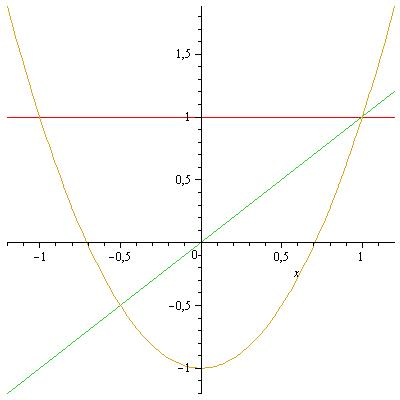
\includegraphics[scale=0.5]{T0T1T2.jpg} \end{center}
Графики многочленов $T_3(x),~ T_4(x),~ T_5(x)$:\begin{center}
    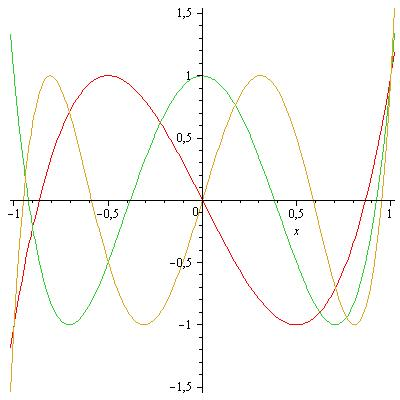
\includegraphics[scale=0.5]{T3T4T5.jpg} \end{center}	
График многочлена $T_{10}(x)$:\begin{center}
    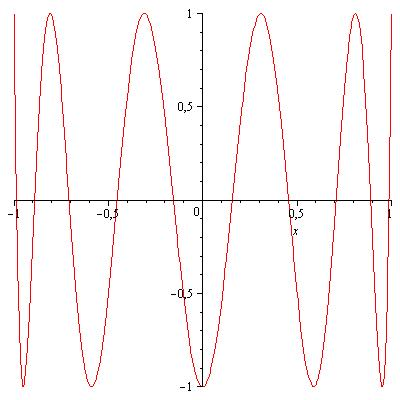
\includegraphics[scale=0.5]{T10.jpg} \end{center} 
\begin{theorem}
    $T_n(cos \varphi)=cos(n\varphi)$
\end{theorem}
\begin{proof}
    \
    \begin{center}
        $x=cos~\varphi$\\
        $cos(2\varphi)=2x^2-1$\\
        $cos(3\varphi)=4x^3-3x$\\
        $\cdots$\\
        $cos(n\varphi)+cos((n-2)\varphi)=2cos \bigg(\cfrac{n+n-2}{2}~\varphi \bigg)cos \bigg(\cfrac{n-n+2}{2}~\varphi \bigg)=2cos((n-1)\varphi)cos \varphi$\\
        ~\\
        $T_n(x)=0 \Leftrightarrow cos(n\varphi)=0 \Leftrightarrow n\varphi=\pi k +\cfrac{\pi}{2}=\pi\cfrac{(2k+1)}{2}, \varphi \in [0, \pi]$\\
        $\varphi=\pi\cfrac{(2k+1)}{2n} \Leftrightarrow x=arccos \bigg(\cfrac{2k+1}{n}~\pi \bigg)$\end{center}
\end{proof}
\begin{consequence}
    \ 
    \begin{itemize}
        \item $T_n(x)=cos(n ~ arccos~x)$ при $ x \in [-1, 1]$
        \item $T_n(x)=\cfrac{(x+\sqrt{x^2-1})^n+(x-\sqrt{x^2-1})^n}{2}$ при $ |x| \geqslant 1$
    \end{itemize}
\end{consequence}

\subsection{Многочлены Чебышева 2 рода}
\begin{definition}
\textbf{Многочленами Чебышева 2 рода} называются следующие многочлены:
\begin{center} $U_n(x)=\cfrac{1}{n+1}T_{n+1}'(x)$ при $ n \geqslant 0$\end{center}
\begin{center}
    \begin{tabular}{|l|l|}
        \hline
        \textbf{n} & \textbf{U(n)} \\ \hline
        0 & 1 \\ \hline
        1 & $2x$ \\ \hline
        2 & $4x^2-1$ \\ \hline
        3 & $8x^3-4x$ \\ \hline
        4 & $16x^4-12x^2+1$ \\ \hline
        5 & $32x^5-32x^3+6x$ \\ \hline
        6 & $64x^6-80x^4+24x^2-1$ \\ \hline
        7 & $128x^7-192x^5+80x^3-8x$ \\ \hline
        8 & $256^8-448x^6+240x^4-40x^2+1$ \\ \hline
        9 & $512x^9-1024x^7+672x^5-160x^3+10x$ \\ \hline
        10 & $1024x^{10}-2304x^8+1792x^6-560x^4+60x^2-1$ \\ \hline
    \end{tabular}
\end{center}
\end{definition} 
Графики многочленов $U_0(x),~ U_1(x),~ U_2(x)$:\begin{center}
    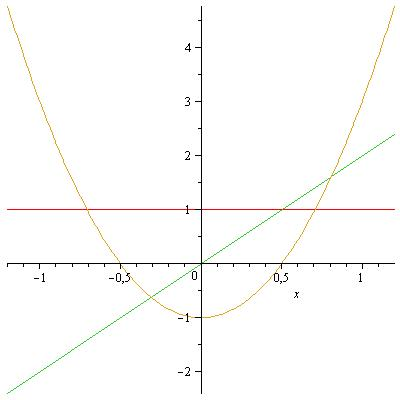
\includegraphics[scale=0.5]{U0U1U2.jpg} \end{center}
Графики многочленов $U_3(x),~ U_4(x),~ U_5(x)$:\begin{center}
    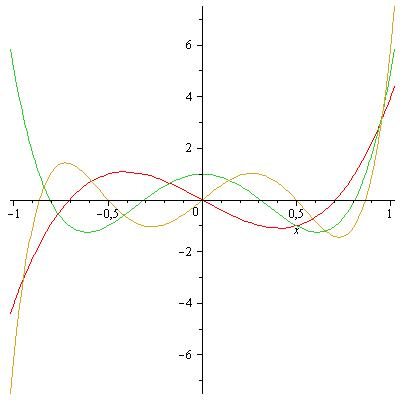
\includegraphics[scale=0.5]{U3U4U5.jpg} \end{center}	
График многочлена $U_{10}(x)$:\begin{center}
    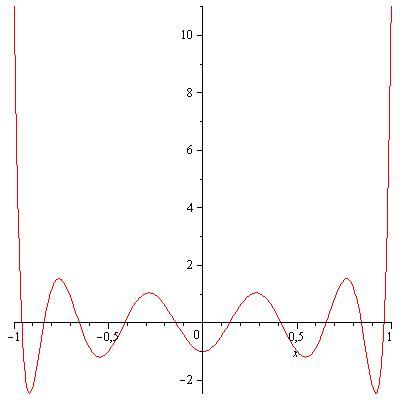
\includegraphics[scale=0.5]{U10.jpg} \end{center}
\begin{theorem}
    \ 
    \begin{enumerate}
        \item $U_{n-1}(cos \varphi)sin \varphi = sin(n \varphi)$
        \item $U_n(x)=\cfrac{(x+\sqrt{x^2-1})^{n+1}+(x-\sqrt{x^2-1})^{n+1}}{\sqrt{x^2-1}}$ при $ |x| \leqslant 1$
    \end{enumerate}
\end{theorem}
\begin{proof}
    \ 
    \begin{enumerate}
        \item $sin(n\varphi)=sin\varphi ~ U_{n-1}(x),$ $ U_{n-1}=\cfrac{sin(n\varphi)}{sin \varphi}$
        \item $U_{n-1}(x) = 0 \Leftrightarrow n\varphi=\pi k,$ $\varphi=\cfrac{\pi k}{n}$
    \end{enumerate}
\end{proof}
\begin{notice}
    Старший коэффициент многочлена $T_n(x)$ равен $2^{n-1}$, а старший коэффициент многочлена $U_n(x)$ равен $2^n$.
\end{notice}
\begin{theorem}
    \ 
    \begin{enumerate}
        \item При $n \geqslant 1$ многочлен $T_n(x)$ имеет на отрезке [-1, 1] ровно $n$ корней $cos\cfrac{(2k-1)\pi}{2n}, k=1,..,n.$
        \item Корни многочлена $U_n(x)$ (они же - экстремумы многочлена $T_{n+1}(x)$) также принадлежат отрезку [-1, 1]: это числа $cos\cfrac{\pi k}{n+1}, k=1,...,n.$
    \end{enumerate}
\end{theorem}
\begin{consequence}
    \ \begin{center}
        $T_n(x)=2^{n-1} \bigg(x-cos~\cfrac{\pi}{2n}\bigg) \bigg(x-cos~\cfrac{3\pi}{2n}\bigg)\cdots \bigg(x-cos(2n-1)\cfrac{\pi}{2n} \bigg)$\\
        ~\\
        $U_n(x)=2^n \bigg(x-cos~\cfrac{\pi}{n+1}\bigg) \bigg(x-cos~\cfrac{2\pi}{n+1} \bigg)\cdots \bigg(x-cos ~n\cfrac{\pi}{n+1}\bigg)$\end{center}
\end{consequence}
\begin{consequence}
    Многочлен $T_n(x)$ степени $n$ на отрезке $[-1, 1]$ достигает своих экстремальных значений, равных 1 и -1 в $n+1$ точке, включая концы отрезка.
\end{consequence}
\textbf{Пример}: $n=6$ (график многочленов $T_6(x)$ и $U_5(x)$).\begin{center}
    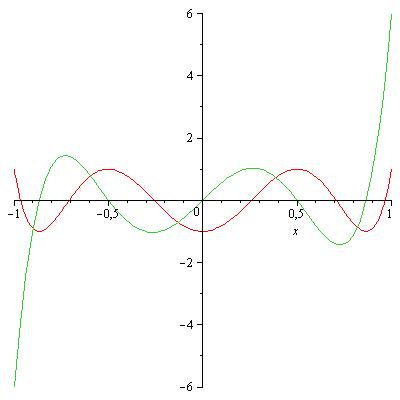
\includegraphics[scale=0.5]{T6U5.jpg} \end{center}
\subsection{Уклонение от нуля и норма Чебышева}
Пусть $f$ --- функция на отрезке $[-1, 1]$. Как измерить, насколько она далека от нуля?
\begin{definition}
Норма Чебышева \begin{center}$|f|_0=\underset{[-1, 1]}{max}|f(x)|$ (максимум модуля на данном отрезке)\end{center}
и \begin{center}$|f|_1=\int\limits_{-1}^1 |f(x)|\,dx$ (площадь под графиком на данном отрезке).\end{center}
\end{definition}
\begin{definition}
Пусть $|| \cdot ||$ --- норма на пространстве многочленов (например, одна из двух упомянутых). Многочлен $f(x)=x^n+\cdots$ степени $n$ со старшим коэффициентом 1 называется \textbf{наименее уклоняющимся от нуля} относительно данной нормы, если для любого другого такого многочлена $g(x)=x^n+\cdots$ всегда $\parallel f \parallel \leqslant \parallel g \parallel$.
\end{definition}
\textbf{Пример 1.}\\
Относительно нормы Чебышева $|f|_0$ уклонение от нуля многочлена $\widetilde{T_3}(x)=\cfrac{1}{4}~T_3(x)=\\=x^3-\cfrac{3}{4}x$ равно\begin{center} $|\cfrac{1}{4}~T_3(x)|_0=\cfrac{1}{4}~|T_3(x)|_0=\cfrac{1}{4}$~,\end{center} а, например, для многочлена $x^3$ имеем $|x^3|_0=1$.\\ \\
\begin{theorem}
    \ 
    \begin{enumerate}
        \item (Чебышев) Наименее уклоняющимся от нуля на отрезке $[-1, 1]$ относительно нормы Чебышева\begin{center} $|f|_0=\underset{[-1, 1]}{max}|f(x)|$ \end{center} является многочлен $\widetilde T_n(x)=\cfrac{1}{2^{n-1}}T_n(x)$.
        \item (Коркин, Золотарев) Наименее уклоняющимся от нуля на отрезке $[-1, 1]$ относительно нормы \begin{center}$|f|_1=\int\limits_{-1}^1 |f(x)|\,dx$ \end{center} является многочлен $\widetilde U_n(x)=\cfrac{1}{2^{n-1}}U_n(x).$
    \end{enumerate}
\end{theorem}
Дано: многочлен $f(x)=x^n+\cdots$ на $[-1, 1]$\\
Надо найти: $g(x)=c \cdot x^n+\cdots$, приближающий $f(x)$ в смысле $|\cdots|_1$ или $|\cdots|_0$.\\
$g \approx f \Leftrightarrow f-g$ --- многочлен, наименее уклоняющийся от нуля, то есть $f(x)-g(x) = \widetilde U_n(x)$ или $\widetilde T_n(x)$.
\begin{consequence}
    Наименее уклоняющийся от нуля на отрезке $[a, b]$ многочлен степени $n$ относительно нормы Чебышева на этом отрезке $|f|_0=\underset{[a, b]}{max}|f(x)|$ --- это \begin{center}$\overline T_n(x) = \cfrac{(b-a)^n}{2^{2n-1}}T_n \bigg(\cfrac{2x-(b+a)}{b-a} \bigg)$.\end{center}
\end{consequence}
\begin{proof}[Идея доказательства]
    Сделать замену переменных $y=\cfrac{2x-(b+a)}{b-a}$, где $x\in [a, b]$, а $y \in [-1, 1]$, и свести задачу к поиску многочлена, наименее уклоняющегося от нуля на отрезке $[-1, 1]$.
\end{proof}
\textbf{Пример 2.}\\
Наименее уклоняющийся от нуля на отрезке $[0, 1]$ многочлен степени $n$ --- это многочлен $$\overline T_n(x)=\cfrac{1}{2^{2n-1}}T_n(2x-1).$$\\
В частности, $\overline T_2(x)=\cfrac{1}{2^{4-1}}T_2(2x-1)=\cfrac{1}{8}(2(2x-1)^2-1)=x^2-x+\cfrac{1}{8}$.
\begin{notice}
\noindent Скалярное произведение непрерывных функций на отрезке $[-1, 1]:$ $$<f, g>=\int\limits_{-1}^1 \cfrac{f(x)g(x)}{\sqrt{1-x^2}}\,dx.$$\\
Ему соответствует норма: $$\parallel f \parallel=\sqrt{<f,f>}=\sqrt{\int\limits_{-1}^1 \cfrac{f(x)^2}{\sqrt{1-x^2}}\,dx}.$$\\
Соотношения ортогональности: $$<T_m, T_n>=
\left\{  
\begin{array}{ccl}  
0,& m\neq n\\
\cfrac{\pi}{2},& m=n\neq 0\\
\pi,& m=n=0\\  
\end{array}   
\right.  
$$
\\
Наилучшее приближение функции $f$ многочленом степени $\leqslant n:$ $$\widetilde f(x)=\sum\limits_{i=0}^n\cfrac{<T_i, f>}{<T_i, T_i>}T_i(x)$$
\end{notice}
\textbf{Пример 3.}\\
$f(x)=x^3$ на $[-1, 1]$ разложить в ряд по многочленам Чебышева.
\begin{center}
    \begin{tabular}{|l|l|}
        \hline
        T & K \\ \hline
        1 & 1 \\ \hline
        $x$ & $x$ \\ \hline
        $2x^2-1$ & $x^2-\frac{1}{2}$ \\ \hline
        $4x^3-3x$ & $x^3-\frac{3}{4}x$\\ \hline
    \end{tabular}
\end{center}
$K=\widetilde T$ --- отнормированные значения.\begin{center}
    $f(x)=x^3=\widetilde T_3+\cfrac{3}{4}\title{T_1}$\\
    $x^3=\sum\limits_{i=0}^3\cfrac{<\widetilde T_i, f>}{<\widetilde T_i, \widetilde T_i>}\widetilde T_i$
\end{center}
\textbf{Пример 4.}\\
$\parallel x^3-P_2(x) \parallel_\infty \to min$ на отрезке $[-1, 1]$ приблизить многочленом, где $P_2(x)$ --- любой многочлен второй степени.\\
\\
Для отрезка $[-1, 1]$: \begin{center}
    $x^3-P_2(x)=\widetilde T_3(x)$\\
    $x^3-x^3+\cfrac{3}{4}x=P_2(x)$\\
    $P_2(x)=\cfrac{3}{4}x$
\end{center}
\textbf{Пример 5.}\\
$\parallel x^3-P_2(x) \parallel_\infty \to min$ на отрезке $[2, 3]$ приблизить многочленом, где $P_2(x)$ --- любой многочлен второй степени.\\
\begin{center}
    $x^3-P_2(x)=\overline T_3(x)$\\
    $P_2(x)=x^3-\overline T_3(x)$\\
\end{center}
Вычислим $\overline T_3(x)$ по формуле $\overline T_n(x) = \cfrac{(b-a)^n}{2^{2n-1}}T_n \bigg(\cfrac{2x-(b+a)}{b-a} \bigg)$.\\
\begin{center}
    $\overline T_3(x)=\cfrac{(b-a)^3}{2^5}T_3 \bigg(\cfrac{2x-(b+a)}{b-a}\bigg) =\cfrac{1}{2^5}T_3(2x-5)=\cfrac{1}{32}(4(2x-5)^3-3(2x-5))=$\\
    $=\cfrac{1}{32}(4(8x^3-60x^2+150x-125)-6x+15)=\cfrac{1}{32}(32x^3-240x^2+600x-500-6x+15)=$\\
    $=x^3-7.5x^2+18.5625x-15.15625$\end{center}
Подставив $\overline T_3(x)$ в $P_2(x)$, получим:
$$P_2(x)=x^3-\overline T_3(x)=7.5x^2-18.5625x+15.15625$$ 
\textbf{Пример 6.}\\
Если $U_n(x)=\cfrac{1}{n+1} \Big(T_{n+1}(x)\Big)'$ будет ли верно $U_{n+1}(x)=2xU_n(x)-U_{n-1}(x)$ ?
\begin{description} 
    \item[n:]
    $$\cfrac{1}{n+1}\Big(2xT_n(x)-T_{n-1}(x)\Big)'=\cfrac{1}{n+1}\Big(2T_n(x)+2xT_n(x)'-T_{n-1}(x)'\Big)$$
    \item[n+1:]
    $$\cfrac{1}{n+2}\Big(2T_{n+1}(x)+2xT_{n+1}(x)'-T_n(x)'\Big)$$
    \item[n-1:]
    $$\cfrac{1}{n}\Big(2T_{n-1}(x)+2xT_{n-1}(x)'-T_{n-2}(x)'\Big)$$
\end{description}
Подставим:
$$\cfrac{2T_{n+1}+2xT_{n+1}'-T_n'}{n+2} \overset{?}{=}\cfrac{2x\Big(2T_n+2xT_n'-T_{n-1}'\Big)}{n+1}-\cfrac{2T_{n-1}+2xT_{n-1}'-T_{n-2}'}{n}$$
\subsection{Домашнее задание 6}
\begin{enumerate}
    \item
    Доказать, что $U_1(x)+U_3(x)+\dots+U_{2n-1}(x)=U_{n-1}(x)U_n(x).$
    \item
    Доказать, что $U_0(x)+U_2(x)+\dots+U_{2n-2}(x)=U_{n-1}^2(x).$
    \item 
    а)Введем на множестве многочленов $\mathbb{R} [x]_{<n}$ 
    степени меньше $n$ от одной переменной скалярное произведение
    $$
    \langle f,g
    \rangle_n
    = \sum\limits_{j=0}^{n-1} f(x_i) g(x_i),
    $$
    где $x_0, \dots,x_{n-1}$ --- нули многочлена Чебышева степени $n$.
    Докажите, что многочлены Чебышева $T_0, \dots, T_{n-1}$ ортогональны друг другу относительно этого скалярного произведения, причем $\langle T_j,T_j
    \rangle_n = n/2$ при $j>0$ и $\langle T_0,T_0
    \rangle_n = n$.\\ \\
    б) Пусть $f$ --- произвольная действительная функция. Предположим, что 
    $P(x)$ --- такой многочлен степени $n$, что 
    $$P(x_m)=
    \sum\limits_{j=0}^{n-1}\cfrac{\langle \hat T_j, f\rangle_n}{\langle \hat T_j, \hat T_j\rangle_n}~\hat T_j(x_m)$$
    для всех $m=0,\dots,n-1$. 
    Докажите, что $P(x)$  является интерполяционным многочленом Лагранжа функции $f$ с узлами в точках $x_0, \dots,x_{n-1}$. 
    \item
    Для $f(x)=x^x$ найти наилучшее линейное приближение на отрезке $[1, 4]$ в норме $\underset{[1, 4]}{max}|f(x)|$.
\end{enumerate}
